%\documentclass[notitlepage,superscriptaddress, 10pt, one-column]{revtex4-1} 
%\documentclass[reprint,...]{revtex4-1} 
%\documentclass[aps,superscriptaddress,twocolumn, pre,showpacs]{revtex4-1}
%\documentclass[aps,superscriptaddress,twocolumn, prl,showpacs]{revtex4-1}
\documentclass[prl,amsmath,twocolumn,nofootinbib]{revtex4}
%\documentclass[aps,superscriptaddress,preprint, pre,showpacs]{revtex4-1}
%\usepackage{acrofont}%NOTE: Comment out this line for the release version!

\usepackage{float}
\usepackage{placeins}
\usepackage{amsmath}
\usepackage{color}
\usepackage{amssymb}
\usepackage{mathtools}
\usepackage{subfigure}
\usepackage{epsfig}
\usepackage{listings}
\usepackage{enumitem}
\usepackage{graphicx}    
\usepackage{graphics}
\usepackage{epstopdf}
\usepackage[pdftex]{hyperref}
\usepackage{breakurl}
\usepackage{epigraph}
\usepackage{xspace}
\usepackage{amsfonts}
\usepackage{eurosym}
\usepackage{ulem}
\usepackage{footmisc}
\usepackage{comment}
\usepackage{caption}
\usepackage{pdflscape}
\usepackage{array}
\usepackage{tikz}
\usetikzlibrary{snakes}
\usetikzlibrary{patterns}

\newcommand{\elabel}[1]{\label{eq:#1}}
\newcommand{\eref}[1]{Eq.~(\ref{eq:#1})}
\newcommand{\ceref}[2]{(\ref{eq:#1}#2)}
\newcommand{\Eref}[1]{Equation~(\ref{eq:#1})}

\newcommand{\Sref}[1]{Section~\ref{sec:#1}}
\newcommand{\sref}[1]{Sec.~\ref{sec:#1}}

\newcommand{\Pref}[1]{Proposition~\ref{prop:#1}}
\newcommand{\pref}[1]{Prop.~\ref{prop:#1}}

\newcommand{\etal}{{\it et~al.}\xspace}
\newcommand{\ie}{{\it i.e.}\ }
\newcommand{\eg}{{\it e.g.}\ }
\newcommand{\etc}{{\it etc.}\ }
\newcommand{\cf}{{\it c.f.}\ }
\newcommand{\ave}[1]{\left\langle#1 \right\rangle}
\newcommand{\person}[1]{{\it \sc #1}}

\newcommand{\OP}[1]{{\it OP: #1 OP}}
\newcommand{\YB}[1]{{\it YB: #1 YB}}

\newcommand{\flabel}[1]{\label{fig:#1}}
\newcommand{\fref}[1]{Fig.~\ref{fig:#1}}
\newcommand{\Fref}[1]{Figure ~\ref{fig:#1}}

\newcommand{\be}{\begin{equation}}
\newcommand{\ee}{\end{equation}}
\newcommand{\bea}{\begin{eqnarray*}}
\newcommand{\eea}{\end{eqnarray*}}

\newcommand{\bi}{\begin{itemize}}
\newcommand{\ei}{\end{itemize}}

\newcommand{\Dt}{\Delta t}
\newcommand{\etau}{\tau^\text{eqm}}
\newcommand{\wtau}{\widetilde{\tau}}
\newcommand{\xN}{\ave{x}_N}
\newcommand{\Sdata}{S^{\text{data}}}
\newcommand{\Smodel}{S^{\text{model}}}

\epstopdfsetup{outdir=./}

\newtheorem{theorem}{Theorem}
\newtheorem{corollary}[theorem]{Corollary}
\newtheorem{proposition}{Proposition}
\newenvironment{proof}[1][Proof]{\noindent\textbf{#1.} }{\ \rule{0.5em}{0.5em}}

\newtheorem{hyp}{Hypothesis}
\newtheorem{subhyp}{Hypothesis}[hyp]

\numberwithin{equation}{section}
\DeclareMathOperator\erf{erf}
\let\endtitlepage\relax

\begin{document}
\title{Measures of intergenerational mobility in a bivariate normal model}
% 
\author{Yonatan Berman}
\email{yonatanb@post.tau.ac.il}
\affiliation{School of Physics and Astronomy, Tel-Aviv University, Tel-Aviv, Israel}

\date{\today}

\begin{abstract} 
We model the joint log-income distribution of parents and children and derive analytic expressions for canonical relative and absolute intergenerational mobility measures. We find that the both types of mobility measures can be expressed as a function of the other.
\end{abstract}

\maketitle

For the past several decades, many scholars have been studying economic intergenerational mobility~\cite{mazumder2005fortunate,aaronson2008intergenerational,lee2009trends,hauser2010intergenerational,corak2013income,chetty2014united}. The motivation for studying mobility stems from its relationship to concepts like equality of opportunity~\cite{roemer2000opportunity,chetty2014land} and the so-called ``American Dream''~\cite{corak2009chasing,chetty2017fading}. Typically measures of mobility are divided into two categories: relative and absolute. Taking the example of income, relative measures gauge the propensity of individuals to change their position in the income distribution, while absolute measures gauge their propensity to change their income in money terms. A hypothetical economy in which all children have exactly twice the real incomes of their parents would exhibit minimal relative mobility and maximal absolute mobility. Therefore, the precise definitions of quoted mobility measures are important.

Our starting point is a population of $N$ parent-child pairs. We denote by $Y_p^i$ and $Y_c^i$ the incomes of the parent and the child (at the same age), respectively, for family $i=1\dots N$. We assume the incomes are all positive and move to define the log-incomes $X_p^i=\log Y_p^i$ and $X_c^i=\log Y_c^i$.

The canonical measure of relative mobility is the elasticity of child income with respect to parent income, known as the intergenerational earnings elasticity (IGE)~\cite{mulligan1997parental,lee2009trends,chetty2014land} and defined as the slope ($\beta$) of the linear regression

\be
X_c = \alpha + \beta X_p + \epsilon\,,
\ee
where $\alpha$ is the regression intercept and $\epsilon$ is the error term.

IGE is a measure of immobility rather than of mobility: the larger it is, the stronger the relationship between the parent and child income. Therefore, $1-\beta$ is often used as a measure of mobility. Empirical studies of IGE and other relative mobility measures in the United States show it holding stable over the past several decades~\cite{lee2009trends,hauser2010intergenerational,chetty2014land,chetty2014united}.

A standard approach to measure absolute intergenerational mobility, recently used in~\cite{chetty2017fading} for studying the trends in absolute mobility in the United States is to measure the fraction of children earning more than their parents, denoted by $A$:

\be
A = \frac{\sum_{j=1}^{N}{1_{\left\{i:Y_c^i>Y_p^i\right\}}\left(Y_c^j\right)}}{N}\,,
\ee
where $1_S\left(x\right)$ is the indicator function for a set $S$ and argument $x$ and $\left\{i:Y_c^i>Y_p^i\right\}$ is the set of children earning more than their parents.

Since the logarithmic function preserves order we also get,

\be
A = \frac{\sum_{j=1}^{N}{1_{\left\{i:X_c^i>X_p^i\right\}}\left(X_c^j\right)}}{N}\,.
\ee

One hypothetical sample of such distribution is presented in~\fref{lines}. It also depicts graphically how $A$ and $\beta$ are defined. The blue line is $y=x$, hence the rate of  absolute mobility is defined as the fraction of parent-child pairs which are above it. The red line is the linear regression $y=\alpha +\beta x$, for which $\beta$ is the IGE.

\begin{figure}[!htb]
\centering
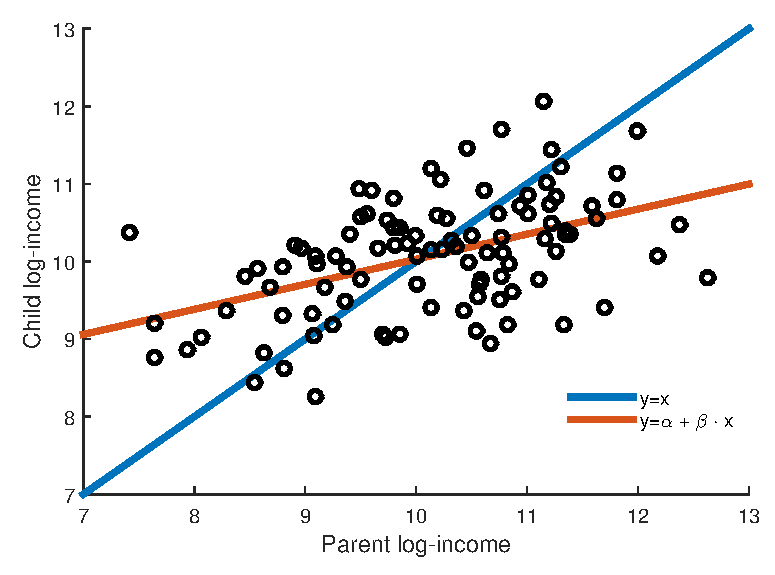
\includegraphics[width=0.5\textwidth]{./figs/bivariate_lines3.eps}
\caption{An illustration of the absolute and relative mobility measures. The black circles are a randomly chosen sample of 100 parent-child log-income pairs. The sample was created assuming a bivariate normal distribution and the parameters used were $\mu_p=10.1$, $\sigma_p=0.78$ (for the parents marginal distribution) and $\mu_c=10.25$, $\sigma_c=1.15$ (for the children marginal distribution) with correlation of $\rho=0.57$. The resulting $\alpha$ and $\beta$ were $1.8$ and $0.84$, respectively.}
\flabel{lines}
\end{figure}

Income distributions are known to be well approximated by the log-normal distribution~\cite{pinkovskiy2009parametric}. Therefore, the minimal plausible model for the joint distribution of parent and child log-incomes is the bivariate normal distribution, in which both marginal income distributions for parents and children are log-normal and the correlation between parent and child incomes is characterized by a single parameter $\rho$. The marginal log-income distribution of the parents (children) follows $\mathcal{N}\left(\mu_p,\sigma_p^2\right)$ ($\mathcal{N}\left(\mu_c,\sigma_c^2\right)$), hence the joint distribution is fully characterized by 5 parameters: $\mu_p$, $\sigma_p$, $\mu_c$, $\sigma_c$ and $\rho$.

Assuming the bivariate normal approximation for the joint distribution enables theoretically studying its properties. In particular Both measures of mobility, $A$ and $1-\beta$, can be derived directly from the model and, notably, can both be expressed analytically as functions of the other. We first derive the IGE in terms of the distribution parameters:

\begin{proposition}
\label{prop:prop1}

For a bivariate normal distribution with parameters $\mu_p$, $\sigma_p$ (for the parents marginal distribution) and $\mu_c$, $\sigma_c$ (for the children marginal distribution) assuming correlation $\rho$, the IGE is

\be
1-\beta = 1-\frac{\sigma_c}{\sigma_p}\rho \,.
\elabel{beta_rho}
\ee
\end{proposition}

\begin{proof}
First, by definition, the correlation $\rho$, between $X_p$ and $X_c$ equals to their covariance, divided by $\sigma_p\sigma_c$

\be
\rho = \frac{\text{Cov}\left[X_p,X_c\right]}{\sigma_p\sigma_c}\,.
\ee

$\beta$ can be directly calculated as follows, by the linear regression slope definition:

\be
\beta = \frac{\sum_{i=1}^{N} {\left(X_p^i - \bar{X}_p\right)\left(X_c^i - \bar{X}_c\right)}}{\sum_{i=1}^{N} {\left(X_p^i - \bar{X}_p\right)}}\,,
\ee
where $\bar{X}_p$ and $\bar{X}_c$ are the average parents and children log-incomes, respectively.

It follows that 
\be
\beta = \frac{\text{Cov}\left[X_p,X_c\right]}{\sigma_p^2}\,.
\ee

We immediately obtain

\be
\beta = \frac{\sigma_c}{\sigma_p}\rho
\ee

and therefore

\be
1-\beta = 1-\frac{\sigma_c}{\sigma_p}\rho
\ee
\end{proof}

Following \pref{prop1} it is also possible to derive the rate of absolute mobility as a function of the distribution parameters and the IGE:

\begin{proposition}
\label{prop:prop2}

For a bivariate normal distribution with parameters $\mu_p$, $\sigma_p$ (for the parents marginal distribution), $\mu_c$, $\sigma_c$ (for the children marginal distribution) and $\rho=\sigma_p\beta/\sigma_c$ (where $\beta$ is the IGE), the rate of absolute mobility is

\be
A = \Phi\left(\frac{\mu_c - \mu_p}{\sqrt{\sigma_p^2\left(1 - 2\beta\right) + \sigma_c^2}}\right) \,,
\elabel{abs2}
\ee
where $\Phi$ is the cumulative distribution function of the standard normal distribution.
\end{proposition}

\begin{proof}
We start by defining a new random variable $Z = X_c-X_p$. It follows that calculating $A$ is equivalent to calculate the probability $P\left(Z>0\right)$.

By definition $Z \sim \mathcal{N}\left(\mu_c - \mu_p,\sigma_p^2 + \sigma_c^2 - 2\text{Cov}\left[X_p,X_c\right]\right)$, so according to \pref{prop1}

\be
Z \sim \mathcal{N}\left(\mu_c - \mu_p,\sigma_p^2\left(1-2\beta\right) + \sigma_c^2\right)\,.
\ee

If follows that

\be
\frac{Z - \left(\mu_c - \mu_p\right)}{\sqrt{\sigma_p^2\left(1-2\beta\right) + \sigma_c^2}} \sim \mathcal{N}\left(0,1\right)\,,
\ee

so we can now write

\be
\begin{split}
&P\left(Z>0\right) = \\ & P\left(\frac{Z - (\mu_c - \mu_p)}{\sqrt{\sigma_p^2\left(1-2\beta\right) + \sigma_c^2}} > -\frac{\mu_c - \mu_p}{\sqrt{\sigma_p^2\left(1-2\beta\right) + \sigma_c^2}} \right) = \\ &\Phi\left(\frac{\mu_c - \mu_p}{\sqrt{\sigma_p^2\left(1 - 2\beta\right) + \sigma_c^2}}\right) \,,
\end{split}
\ee
where $\Phi$ is the cumulative distribution function of the standard normal distribution.

\end{proof}

\Pref{prop2} shows that the rate of absolute mobility can be explicitly described as a function of the relative mobility.

\bibliographystyle{plain}
\bibliography{mobmob}

\end{document}